\documentclass[a4paper,11pt]{article}
\usepackage[margin=22mm,top=25mm,bottom=25mm]{geometry}
\usepackage{fontspec}
\usepackage{xcolor}
\usepackage{booktabs}
\usepackage{tabularx}
\usepackage{colortbl}
\usepackage{multirow}
\usepackage{graphicx}
\usepackage{tikz}
\usetikzlibrary{matrix,positioning,calc,arrows.meta}
\usepackage{enumitem}
\usepackage{fancyhdr}
\usepackage{hyperref}
\usepackage{amssymb}

% Fonts — fallback to system fonts
\setmainfont{Helvetica Neue}
\setmonofont{Menlo}[Scale=0.85]

% Ainary CI Colors
\definecolor{gold}{HTML}{c8aa50}
\definecolor{warmgold}{HTML}{d4a853}
\definecolor{deepgold}{HTML}{9d7f3b}
\definecolor{palegold}{HTML}{e8d89f}
\definecolor{bg}{HTML}{fafaf8}
\definecolor{surface}{HTML}{ffffff}
\definecolor{textprimary}{HTML}{1a1a1a}
\definecolor{textsecondary}{HTML}{666666}
\definecolor{border}{HTML}{e5e5e0}

% Risk colors
\definecolor{riskred}{HTML}{dc3545}
\definecolor{riskorange}{HTML}{fd7e14}
\definecolor{riskyellow}{HTML}{ffc107}
\definecolor{riskgreen}{HTML}{28a745}
\definecolor{riskredlight}{HTML}{fde8ea}
\definecolor{riskorangelight}{HTML}{fff3e0}
\definecolor{riskyellowlight}{HTML}{fff9e6}
\definecolor{riskgreenlight}{HTML}{e8f5e9}
\definecolor{riskgray}{HTML}{f8f9fa}

% Header
\pagestyle{fancy}
\fancyhf{}
\renewcommand{\headrulewidth}{0.5pt}
\renewcommand{\headrule}{\hbox to\headwidth{\color{gold}\leaders\hrule height \headrulewidth\hfill}}
\fancyhead[L]{\footnotesize\color{textsecondary}RISIKOANALYSE · Lagerungstraverse KBA}
\fancyhead[R]{\footnotesize\color{textsecondary}INTERN · 2026-02-10}
\fancyfoot[C]{\footnotesize\color{textsecondary}\thepage}
\fancyfoot[R]{\footnotesize\color{textsecondary}CNC Planner Pro}

\setlength{\parindent}{0pt}
\setlength{\parskip}{6pt}

% Custom commands
\newcommand{\sectiongold}[1]{%
  \vspace{14pt}%
  {\Large\bfseries\color{textprimary}#1}\\[-4pt]%
  {\color{gold}\rule{\textwidth}{2pt}}%
  \vspace{6pt}%
}
\newcommand{\subsectiongold}[1]{%
  \vspace{8pt}%
  {\large\bfseries\color{textprimary}#1}\\[-4pt]%
  {\color{border}\rule{0.5\textwidth}{0.5pt}}%
  \vspace{4pt}%
}

\newcommand{\circled}[1]{%
  \tikz[baseline=(char.base)]{
    \node[shape=circle,draw=deepgold,fill=palegold!30,inner sep=1.5pt,font=\footnotesize\bfseries] (char) {#1};
  }%
}

\newcommand{\riskbadge}[2]{%
  \tikz[baseline=(badge.base)]{
    \node[fill=#1,text=white,rounded corners=2pt,inner sep=2pt,font=\footnotesize\bfseries] (badge) {#2};
  }%
}

\begin{document}

% ============================================================
% TITLE
% ============================================================
\thispagestyle{empty}
\begin{center}
\vspace*{20mm}

{\color{gold}\rule{\textwidth}{2pt}}
\vspace{8mm}

{\fontsize{28}{34}\selectfont\bfseries\color{textprimary}RISIKOANALYSE}\\[4mm]
{\fontsize{16}{20}\selectfont\color{textsecondary}Kalkulation Lagerungstraverse}\\[2mm]
{\fontsize{14}{18}\selectfont\color{textsecondary}Zeichnung 10028104.79 · KBA Koenig \& Bauer}

\vspace{8mm}
{\color{gold}\rule{\textwidth}{2pt}}

\vspace{20mm}

\begin{tabular}{ll}
\color{textsecondary}Basiskalkulation: & \textbf{EUR 19.730 / Stück} \\[3pt]
\color{textsecondary}Bandbreite: & \textbf{EUR 14.200 – 26.800} \\[3pt]
\color{textsecondary}Confidence: & \textbf{75\% (Mittel-Hoch)} \\[3pt]
\color{textsecondary}Stückzahl: & 4 Stück \\[3pt]
\color{textsecondary}Datum: & 2026-02-10 \\
\end{tabular}

\vspace{30mm}

\fcolorbox{riskorange}{riskorangelight}{%
  \parbox{0.85\textwidth}{%
    \centering\bfseries\color{riskorange}\large
    ⚠ INTERNES DOKUMENT — NICHT FÜR KUNDEN
  }%
}

\vfill
{\small\color{textsecondary}CNC Planner Pro · AI-Assisted Calculation · Ainary Consulting}
\end{center}

\newpage
\setcounter{page}{1}

% ============================================================
% ZEICHNUNG
% ============================================================
\sectiongold{Technische Zeichnung — Lagerungstraverse 10028104.79}

\vspace{4pt}
{\footnotesize\color{textsecondary}Quelle: KBA Anfrage 6000063225 · Zeichnung 10028104.79 · Maßstab: nicht maßstabsgetreu}

\vspace{8pt}
\begin{center}
\includegraphics[width=\textwidth,keepaspectratio]{/tmp/anfrage_page_0.png}
\end{center}

\vspace{4pt}
{\footnotesize
\begin{tabularx}{\textwidth}{llll}
\textbf{Werkstoff:} S355 / GJS-700 (klärungsbedürftig) & 
\textbf{Maße:} 2095 × 500 × 190 mm & 
\textbf{Stück:} 4 & 
\textbf{Toleranz:} ISO 2768-m \\
\end{tabularx}
}

\newpage

% ============================================================
% FERTIGUNGSANWEISUNG
% ============================================================
\sectiongold{Fertigungsanweisung — Operationsplan}

\vspace{4pt}
{\footnotesize\color{textsecondary}Vorschlag auf Basis REFA/VDI 3321 · Abgleich mit betrieblicher Erfahrung empfohlen · 4 Aufspannungen}

\vspace{8pt}

\begin{tabularx}{\textwidth}{>{\footnotesize\bfseries}c >{\footnotesize}p{32mm} >{\footnotesize}p{30mm} >{\footnotesize}p{28mm} >{\footnotesize}X >{\footnotesize}r}
\toprule
\textbf{AG} & \textbf{Arbeitsgang} & \textbf{Werkzeug} & \textbf{Parameter} & \textbf{Hinweise} & \textbf{min} \\
\midrule
\rowcolor{riskgray}
\multicolumn{6}{l}{\bfseries\color{deepgold} Aufspannung 1 — Unterseite (Rüsten: 50 min)} \\
10 & Sägen \& Vorbereitung & Bandsäge & -- & Rohteil ablängen 2150mm, Kanten grob entgraten. Rohgewicht ca. 1.856\,kg. & 28 \\
\rowcolor{riskgreenlight}
20 & Planfräsen Unterseite & T1 Ø80 Planfräser & n600 · vf750 · ap2,0 & Referenzfläche 2095×500mm. ae=64mm, 8 Bahnen, Schlichtzugabe 0,2mm. & 55 \\
30 & Bohrungen Unterseite & T2 Ø16 VHM, T3 Ø10 VHM & 8×Ø16 H7, 4×Ø10 H7 & Zentrierung + Bohren + Senken. Ø16: 4min/Bohrung, Ø10: 3min/Bohrung. & 44 \\
\midrule
\rowcolor{riskgray}
\multicolumn{6}{l}{\bfseries\color{deepgold} Aufspannung 2 — Oberseite (Rüsten: 38 min)} \\
\rowcolor{riskgreenlight}
40 & Planfräsen Oberseite & T1 Ø80 Planfräser & n600 · vf750 · ap2,0 & Parallelfläche zu US, Sollmaß 190mm ±0,05. Ra\,3,2. & 52 \\
50 & Taschen fräsen (4×) & T4 Ø20 VHM & n2400 · vf960 · ap4,0 & T1: 400×280 t=50 (18min), T2: 275×180 t=35 (12min), T3/4: 150×100 t=25 (2×8min) & 46 \\
\rowcolor{riskgreenlight}
60 & Langlöcher (3×) & T4 Ø20 VHM & 3× 120×40 durchg. & Vorbohren Ø16 + Ausfräsen = 8min/Langloch. & 24 \\
70 & Konturfräsen Außen & T5 Ø16 VHM & n3000 · vf600 · ap4,0 & Brennschnitt-Zugabe 2mm abtragen. Umfang ca. 6m, 2 Zustellungen. & 28 \\
\midrule
\rowcolor{riskgray}
\multicolumn{6}{l}{\bfseries\color{deepgold} Aufspannung 3 — Stirnseite 1 (Rüsten: 39 min)} \\
80 & Planfräsen + Bohrungen & T1 Ø80, T6 Ø12 VHM & Kontrollmaß 1508 ±0,1 & 500×190mm planfräsen (8min) + 4×Ø12 (8min/Bohrung) & 40 \\
\midrule
\rowcolor{riskgray}
\multicolumn{6}{l}{\bfseries\color{deepgold} Aufspannung 4 — Stirnseite 2 (Rüsten: 37 min)} \\
\rowcolor{riskgreenlight}
90 & Planfräsen + Bohrungen + Gewinde & T1, T6, T7 M16 & Kontrollmaß 1400 ±0,1 & 500×190mm Plan (8min) + 4×Ø12 (8min) + 3×M16 (5min) + Fase (4min) & 57 \\
\midrule
\rowcolor{riskgray}
\multicolumn{6}{l}{\bfseries\color{deepgold} Nachbearbeitung} \\
100 & Entgraten komplett & Handwerkzeug & -- & Alle Kanten, Bohrungen, Taschen. Großteil bei 1,5t → Kran zum Wenden. & 68 \\
\rowcolor{riskgreenlight}
110 & Qualitätsprüfung & Messprotokoll & -- & Alle H7-Bohrungen, Kontrollmaße 1508/1400, Parallelität, Rechtwinkligkeit. & 55 \\
\midrule
\rowcolor{palegold!20}
& \textbf{Σ Bearbeitung} & & & & \textbf{497} \\
\rowcolor{palegold!20}
& \textbf{Σ Rüsten (4 Aufsp.)} & & & & \textbf{164} \\
\rowcolor{palegold!30}
& \textbf{Σ Gesamt pro Stück} & & & & \textbf{661} \\
\bottomrule
\end{tabularx}

\vspace{8pt}
\fcolorbox{gold}{palegold!20}{%
  \parbox{0.95\textwidth}{\footnotesize
    \textbf{661 min = 11,0 Stunden pro Stück.} Realistische Bandbreite: 580 – 790 min (±20\%). 
    Rüstzeit teilt sich auf 4 Stück → Rüstkostenanteil pro Stück = 164 min ÷ 4 = 41 min.
    Schnittdaten-Basis: Sandvik CoroPlus / Walter GPS für S355 (HB\,180).
  }%
}

\newpage

% ============================================================
% EXECUTIVE SUMMARY
% ============================================================
\sectiongold{1 \quad Executive Summary}

Die automatische Kalkulation ergibt \textbf{EUR 19.730/Stück} (netto). Diese Analyse identifiziert die Hauptrisiken und zeigt drei Szenarien mit konkreten Handlungsoptionen.

\vspace{6pt}

\begin{tabularx}{\textwidth}{>{\bfseries}l X r r}
\toprule
\textbf{Szenario} & \textbf{Annahmen} & \textbf{Preis/Stk} & \textbf{vs. Basis} \\
\midrule
\rowcolor{riskgreenlight}
Best Case & GJS-700 Gussteil, 3 Aufspannungen & EUR 14.200 & −28\% \\
\rowcolor{riskgray}
Expected & S355 Blech, Brennschnitt geliefert, 4 Aufsp. & EUR 19.730 & Basis \\
\rowcolor{riskyellowlight}
Konservativ & S355, kein Brennschnitt, CAM separat & EUR 23.500 & +19\% \\
\rowcolor{riskredlight}
Worst Case & Rohplatte, 5 Aufsp., Zeugnis 3.1, Sonderwerkzeuge & EUR 26.800 & +36\% \\
\bottomrule
\end{tabularx}

\vspace{8pt}

\textbf{Kernaussage:} Drei Fragen entscheiden über den Preis:
\begin{enumerate}[leftmargin=*, itemsep=2pt]
  \item \textbf{S355 oder GJS-700?} → Werkstoff ändert Preis um ±50\%
  \item \textbf{Wer liefert das Rohteil?} → Material = 78\% der Kosten
  \item \textbf{Brennschnitt inklusive?} → Ohne Vorschnitt: +EUR 1.200/Stk
\end{enumerate}

% ============================================================
% RISK MATRIX
% ============================================================
\sectiongold{2 \quad Risiko-Matrix}

\begin{center}
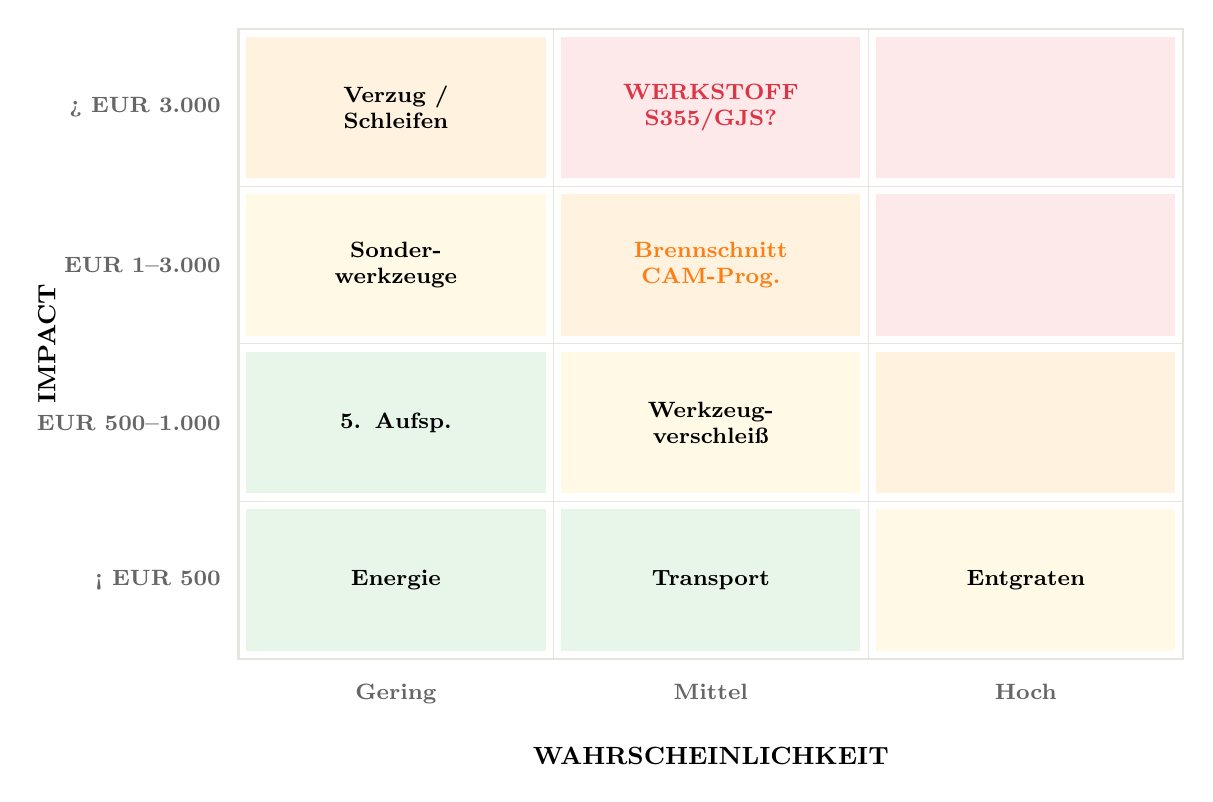
\begin{tikzpicture}[
  cell/.style={minimum width=38mm, minimum height=18mm, text width=35mm, align=center, font=\footnotesize},
  label/.style={font=\footnotesize\bfseries, text=textsecondary},
]

% Grid
\foreach \y/\ylabel/\ycolor in {3/{> EUR 3.000}/riskredlight, 2/{EUR 1–3.000}/riskorangelight, 1/{EUR 500–1.000}/riskyellowlight, 0/{< EUR 500}/riskgreenlight} {
  \foreach \x in {0,1,2} {
    % Darken cells in top-right
    \pgfmathtruncatemacro{\risk}{\x+\y}
    \ifnum\risk>3
      \node[cell, fill=riskredlight] at (\x*40mm, \y*20mm) {};
    \else\ifnum\risk>2
      \node[cell, fill=riskorangelight] at (\x*40mm, \y*20mm) {};
    \else\ifnum\risk>1
      \node[cell, fill=riskyellowlight] at (\x*40mm, \y*20mm) {};
    \else
      \node[cell, fill=riskgreenlight] at (\x*40mm, \y*20mm) {};
    \fi\fi\fi
  }
  \node[label, anchor=east] at (-21mm, \y*20mm) {\ylabel};
}

% X-axis labels
\foreach \x/\xlabel in {0/Gering, 1/Mittel, 2/Hoch} {
  \node[label, anchor=north] at (\x*40mm, -12mm) {\xlabel};
}

% Axis titles
\node[font=\small\bfseries, rotate=90, anchor=south] at (-42mm, 30mm) {IMPACT};
\node[font=\small\bfseries, anchor=north] at (40mm, -20mm) {WAHRSCHEINLICHKEIT};

% Risk items
\node[cell, font=\footnotesize\bfseries] at (0mm, 60mm) {Verzug /\\Schleifen};
\node[cell, font=\footnotesize\bfseries, text=riskred] at (40mm, 60mm) {\textbf{WERKSTOFF}\\S355/GJS?};
\node[cell, font=\footnotesize\bfseries] at (0mm, 40mm) {Sonder-\\werkzeuge};
\node[cell, font=\footnotesize\bfseries, text=riskorange] at (40mm, 40mm) {Brennschnitt\\CAM-Prog.};
\node[cell, font=\footnotesize\bfseries] at (0mm, 20mm) {5. Aufsp.};
\node[cell, font=\footnotesize\bfseries] at (40mm, 20mm) {Werkzeug-\\verschleiß};
\node[cell, font=\footnotesize\bfseries] at (0mm, 0mm) {Energie};
\node[cell, font=\footnotesize\bfseries] at (40mm, 0mm) {Transport};
\node[cell, font=\footnotesize\bfseries] at (80mm, 0mm) {Entgraten};

% Border
\draw[border, thick] (-20mm,-10mm) rectangle (100mm,70mm);
\foreach \y in {0,1,2,3} {
  \draw[border] (-20mm,\y*20mm-10mm) -- (100mm,\y*20mm-10mm);
}
\foreach \x in {0,1,2} {
  \draw[border] (\x*40mm-20mm,-10mm) -- (\x*40mm-20mm,70mm);
}

\end{tikzpicture}
\end{center}

\vspace{4pt}
\textbf{Top 3 Risiken nach Expected Monetary Value:}
\begin{enumerate}[leftmargin=*, itemsep=2pt]
  \item \riskbadge{riskred}{KRITISCH} \textbf{Werkstoff S355 vs. GJS-700:} EMV = 50\% × EUR 8.000 = \textbf{EUR 4.000}
  \item \riskbadge{riskorange}{HOCH} \textbf{Materialpreis-Unsicherheit:} EMV = 40\% × EUR 3.000 = \textbf{EUR 1.200}
  \item \riskbadge{riskyellow}{MITTEL} \textbf{Brennschnitt nicht inklusive:} EMV = 30\% × EUR 1.200 = \textbf{EUR 360}
\end{enumerate}

% ============================================================
% PREISTREIBER
% ============================================================
\sectiongold{3 \quad Preistreiber-Analyse}

\subsectiongold{A — Werkstoff (±EUR 8.000 / Stück)}

\fcolorbox{riskred}{riskredlight}{%
  \parbox{0.95\textwidth}{%
    \textbf{Widerspruch in der Zeichnung:} Der Zeichnungskopf nennt sowohl S355 (Baustahl) als auch GJS-700 (Sphäroguss). Das sind komplett verschiedene Werkstoffe mit verschiedenen Preisen und Rohteilformen.
  }%
}

\vspace{6pt}

\begin{tabularx}{\textwidth}{l X r r r}
\toprule
\textbf{Option} & \textbf{Rohteilform} & \textbf{Material/Stk} & \textbf{FEK/Stk} & \textbf{Gesamt/Stk} \\
\midrule
\rowcolor{riskgray}
\textbf{A1: S355 Blech} & Platte 2150×550×200, ausgebrannt & EUR 13.920 & EUR 924 & \textbf{EUR 19.730} \\
\textbf{A2: GJS-700 Guss} & Gussteil, Aufmaß 3–5mm & EUR 4.000* & EUR 520 & \textbf{EUR 8.500*} \\
\textbf{A3: KBA liefert} & Beistellung Rohteil & EUR 0 & EUR 924 & \textbf{EUR 4.400} \\
\bottomrule
\end{tabularx}

{\footnotesize *Gießerei-Preis geschätzt, abhängig von Modellkosten und Losgröße.}

\subsectiongold{B — Materialpreis S355 (±EUR 3.000 / Stück)}

\begin{tabularx}{\textwidth}{l r r r}
\toprule
\textbf{Quelle} & \textbf{EUR/kg} & \textbf{Rohteil 1.856kg} & \textbf{vs. Basis} \\
\midrule
CNC Planner Demo (Default) & 1,65 & EUR 3.062 & −EUR 10.858 \\
\rowcolor{riskgray}
\textbf{Stahlhandel Q1/2026 (Basis)} & \textbf{7,50} & \textbf{EUR 13.920} & \textbf{---} \\
Thyssen/Klöckner Dickblech & 8,50 & EUR 15.776 & +EUR 1.856 \\
S355J2+N mit Zeugnis 3.1 & 9,20 & EUR 17.075 & +EUR 3.155 \\
\bottomrule
\end{tabularx}

\subsectiongold{C — Brennschnitt (±EUR 1.200 / Stück)}

\begin{tabularx}{\textwidth}{l X r}
\toprule
\textbf{Szenario} & \textbf{Beschreibung} & \textbf{Mehrkosten} \\
\midrule
\rowcolor{riskgreenlight}
Kontur geliefert (Annahme) & Brennschnitt durch KBA oder Zulieferer & EUR 0 \\
\rowcolor{riskyellowlight}
Autogen-Brennschnitt extern & 2095mm Kontur, 200mm Dicke & +EUR 800 \\
\rowcolor{riskorangelight}
Wasserstrahlschnitt extern & Für enge Brennschnitt-Zugabe & +EUR 1.500 \\
\bottomrule
\end{tabularx}

% ============================================================
% HIDDEN COSTS
% ============================================================
\sectiongold{4 \quad Versteckte Kosten (nicht in Basis-Kalkulation)}

\begin{tabularx}{\textwidth}{l X r l}
\toprule
\textbf{Position} & \textbf{Beschreibung} & \textbf{Kosten/Stk} & \textbf{Prio} \\
\midrule
CAM-Programmierung & 4–8h Erstprogramm + Simulation & EUR 225–330* & \riskbadge{riskorange}{HOCH} \\
Werkzeugverschleiß & WSP, VHM-Fräser bei 8h in S355 & EUR 290–430 & \riskbadge{riskorange}{HOCH} \\
Einfahren 1. Teil & +50\% Bearbeitungszeit beim Erstteil & EUR 460* & \riskbadge{riskyellow}{MITTEL} \\
Transport & 4× 1,2t Fertigteile, LKW & EUR 100–250 & \riskbadge{riskgreen}{GERING} \\
Oberflächenbehandl. & Falls Lackierung/KTL gefordert & EUR 0–500 & \riskbadge{riskyellow}{MITTEL} \\
\midrule
\textbf{Summe} & & \textbf{EUR 1.075–1.970} & \\
\bottomrule
\end{tabularx}

{\footnotesize *Bei 4 Stück auf Losgröße umgelegt.}

\vspace{6pt}
\fcolorbox{gold}{palegold!30}{%
  \parbox{0.95\textwidth}{%
    \textbf{Empfehlung:} Diese Positionen im Gewinnzuschlag auffangen (12\% → 15\%) oder als separate Position „Einmalige Einrichtung" im Angebot ausweisen.
  }%
}

% ============================================================
% DECISION MATRIX
% ============================================================
\newpage
\sectiongold{5 \quad Entscheidungsmatrix — Angebotsoptionen}

\renewcommand{\arraystretch}{1.4}
\begin{tabularx}{\textwidth}{>{\bfseries}p{30mm} X X X}
\toprule
& \textbf{Option 1: Pauschal} & \textbf{Option 2: Getrennt} & \textbf{Option 3: Nur Bearbeitung} \\
\midrule
\rowcolor{riskgray}
Beschreibung & Alles-inklusive Stückpreis & Material + Bearbeitung separat & Nur CNC, Kunde stellt Rohteil \\

Preis/Stk & EUR 19.730 & EUR 13.920 (Mat)\newline EUR 5.810 (Bearb) & EUR 5.810 \\

Risiko für uns & \riskbadge{riskred}{HOCH}\newline Materialpreisschwankung & \riskbadge{riskyellow}{MITTEL}\newline Bearbeitungszeit & \riskbadge{riskgreen}{GERING}\newline Nur eigene Leistung \\

Risiko Kunde & \riskbadge{riskgreen}{GERING}\newline Festpreis & \riskbadge{riskyellow}{MITTEL}\newline Mat.-Preis variabel & \riskbadge{riskorange}{HOCH}\newline Muss selbst beschaffen \\

Marge & 12\% (EUR 2.114) & 12\% auf Bearb.\newline 5\% auf Material & 15\% (EUR 760) \\

\rowcolor{riskgray}
Empfehlung & Bei stabilen Mat.-Preisen und Serienauftrag & \cellcolor{riskgreenlight}\textbf{EMPFOHLEN}\newline Transparent, flexibel & Bei Kunden-Beistellung \\
\bottomrule
\end{tabularx}
\renewcommand{\arraystretch}{1.0}

\vspace{12pt}

\subsectiongold{Staffelpreise (Option 2 — Getrennt)}

\begin{tabularx}{\textwidth}{r r r r r r}
\toprule
\textbf{Stück} & \textbf{Material} & \textbf{Bearbeitung} & \textbf{Einrichtung*} & \textbf{Stückpreis} & \textbf{Gesamt netto} \\
\midrule
1 & 13.920 & 5.810 & 900 & \textbf{20.630} & 20.630 \\
\rowcolor{riskgray}
\textbf{4} & \textbf{13.920} & \textbf{5.500} & \textbf{225} & \textbf{19.645} & \textbf{78.580} \\
5 & 13.920 & 5.400 & 180 & 19.500 & 97.500 \\
10 & 13.770 & 5.100 & 90 & 18.960 & 189.600 \\
\bottomrule
\end{tabularx}

{\footnotesize *Einrichtung = CAM-Programmierung + Einfahren, umgelegt auf Losgröße.}

% ============================================================
% ACTION ITEMS
% ============================================================
\sectiongold{6 \quad Vor Angebotsabgabe klären}

\begin{tabularx}{\textwidth}{c l X r}
\toprule
\textbf{Prio} & \textbf{\#} & \textbf{Frage an KBA} & \textbf{Impact} \\
\midrule
\riskbadge{riskred}{1} & A1 & \textbf{Welcher Werkstoff: S355 oder GJS-700?} & ±EUR 8.000 \\
\riskbadge{riskred}{1} & A2 & \textbf{Rohteil-Beistellung oder Beschaffung durch uns?} & ±EUR 13.920 \\
\riskbadge{riskred}{1} & A3 & \textbf{Ist Kontur bereits ausgebrannt/gelasert?} & ±EUR 1.200 \\
\rowcolor{riskgray}
\riskbadge{riskorange}{2} & B1 & 3D-Modell (STEP) verfügbar? & Genauigkeit \\
\riskbadge{riskorange}{2} & B2 & Welche Dokumentation? (Messprotokoll, Zeugnis) & ±EUR 500 \\
\riskbadge{riskorange}{2} & B3 & Oberflächenbehandlung gefordert? & ±EUR 500 \\
\riskbadge{riskyellow}{3} & C1 & Gewünschte Lieferzeit? & Planung \\
\riskbadge{riskyellow}{3} & C2 & Lieferadresse (Sondertransport?) & ±EUR 500 \\
\bottomrule
\end{tabularx}

\vspace{12pt}

\subsectiongold{Werker-Validierung (intern)}

\begin{tabularx}{\textwidth}{X r}
\toprule
\textbf{Frage an erfahrenen Werker} & \textbf{Validiert} \\
\midrule
Tischspannung 2m-Teil, 1,5t — wie lange? (Annahme: 35min) & $\square$ \\
Planfräsen 2095×500mm in S355 mit Ø80 — unter 60min? (Annahme: 55min) & $\square$ \\
4 Aufspannungen realistisch oder geht es mit 3? & $\square$ \\
Werkzeugverbrauch bei 8h S355? WSP-Sätze pro Teil? & $\square$ \\
Entgraten komplett — 1h realistisch? (Annahme: 68min) & $\square$ \\
\bottomrule
\end{tabularx}

% ============================================================
% OPTIMALER WORKFLOW — 1-Pager
% ============================================================
\newpage
% ============================================================
% ANHANG A: DETAILBERECHNUNG PRO ARBEITSGANG
% ============================================================
\sectiongold{7 \quad Detailberechnung — Arbeitsgänge mit Bandbreiten}

{\footnotesize\color{textsecondary}Alle Zeiten in Minuten. Formeln nach REFA / VDI 3321. Schnittdaten nach Sandvik CoroPlus (S355, HB 180).}

\vspace{6pt}

\subsectiongold{AG 1 — Sägen \& Vorbereitung}

\begin{tabularx}{\textwidth}{>{\footnotesize}l >{\footnotesize}X >{\footnotesize}r >{\footnotesize}r >{\footnotesize}r}
\toprule
\textbf{Schritt} & \textbf{Berechnung} & \textbf{Best} & \textbf{Erw.} & \textbf{Worst} \\
\midrule
Rüsten & Material bereitstellen, Anschlag & 10 & 15 & 20 \\
\rowcolor{riskgray}
Sägen & $t_h = \frac{B}{v_f} = \frac{550\text{mm}}{70\text{mm/min}} \approx 8\text{min}$ & 6 & 8 & 12 \\
Entgraten grob & Schnittkanten, manuell & 3 & 5 & 8 \\
\midrule
\textbf{Gesamt AG 1} & \textbf{Satz: EUR 45/h (Sägen)} & \textbf{19} & \textbf{28} & \textbf{40} \\
\textbf{Kosten} & & \textbf{EUR 14} & \textbf{EUR 21} & \textbf{EUR 30} \\
\bottomrule
\end{tabularx}

{\footnotesize\color{textsecondary}
⚠ \textbf{Unsicherheit:} Säge-Typ unbekannt (Bandsäge vs. Kreissäge). Bei Bandsäge +50\% Sägezeit. Annahme: Bandsäge mit Hartmetall-Band.}

\vspace{8pt}
\subsectiongold{AG 2 — CNC Aufspannung 1 (Unterseite)}

\textbf{Rüstzeit:}
\begin{tabularx}{\textwidth}{>{\footnotesize}l >{\footnotesize}X >{\footnotesize}r >{\footnotesize}r >{\footnotesize}r}
\toprule
\textbf{Position} & \textbf{Herleitung} & \textbf{Best} & \textbf{Erw.} & \textbf{Worst} \\
\midrule
Pratzen setzen & 2095mm Teil, 6 Pratzen, Kran nötig (1,5t) & 25 & 35 & 45 \\
\rowcolor{riskgray}
WZ einwechseln & 3 Werkzeuge × 2–3 min & 6 & 8 & 10 \\
Nullpunkt tasten & Messtaster, Referenzbohrung & 5 & 7 & 10 \\
\midrule
\textbf{Rüstzeit Aufsp. 1} & & \textbf{36} & \textbf{50} & \textbf{65} \\
\bottomrule
\end{tabularx}

\vspace{4pt}
\textbf{Bearbeitungsschritte:}
\begin{tabularx}{\textwidth}{>{\footnotesize}l >{\footnotesize}X >{\footnotesize}r >{\footnotesize}r >{\footnotesize}r}
\toprule
\textbf{Schritt} & \textbf{Formel / Herleitung} & \textbf{Best} & \textbf{Erw.} & \textbf{Worst} \\
\midrule
\rowcolor{riskgray}
Planfräsen & $n_{Bahnen} = \frac{500}{0{,}8 \times 80} = 8$ Bahnen & & & \\
2095×500mm & $t_h = \frac{2095 \times 8}{750} \times 1{,}15 = 55\text{min}$ & 42 & 55 & 68 \\
\rowcolor{riskgray}
& $v_c=150$, $f_z=0{,}15$, $a_p=2$, Ø80 Planfräser & & & \\
\midrule
Bohrungen 8×Ø16 & Pro Bohrung: Zentr. 1' + Bohren 3' + Senken 0,5' & 24 & 32 & 42 \\
\rowcolor{riskgray}
H7, t=190mm & $t_h = \frac{L}{f \times n} = \frac{190}{0{,}15 \times 1200} \approx 1\text{min}$ (×2 Stufen) & & & \\
\midrule
Referenzbohrun- & 4× Ø10 H7, Präzision & 8 & 12 & 16 \\
gen (Messtaster) & & & & \\
\midrule
\textbf{Bearb. Aufsp. 1} & & \textbf{74} & \textbf{99} & \textbf{126} \\
\textbf{Gesamt AG 2} & \textbf{Satz: EUR 70/h (CNC)} & \textbf{110} & \textbf{149} & \textbf{191} \\
\textbf{Kosten} & & \textbf{EUR 128} & \textbf{EUR 174} & \textbf{EUR 223} \\
\bottomrule
\end{tabularx}

{\footnotesize\color{textsecondary}
⚠ \textbf{Unsicherheit Planfräsen:} Fräser-Ø (63/80/100?) ändert Bahnanzahl. Ø100 → 5 Bahnen → 35min. \\
⚠ \textbf{Unsicherheit Bohrungen:} Tiefe 190mm = 12×D bei Ø16 → ggf. Tiefbohrverfahren nötig (+50\% pro Bohrung).}

\vspace{8pt}
\subsectiongold{AG 3 — CNC Aufspannung 2 (Oberseite)}

\textbf{Rüstzeit:}
\begin{tabularx}{\textwidth}{>{\footnotesize}l >{\footnotesize}X >{\footnotesize}r >{\footnotesize}r >{\footnotesize}r}
\toprule
\textbf{Position} & \textbf{Herleitung} & \textbf{Best} & \textbf{Erw.} & \textbf{Worst} \\
\midrule
Teil wenden & Kran, Folgeaufsp. (Setup bekannt) & 15 & 21 & 28 \\
\rowcolor{riskgray}
WZ einwechseln & 5 Werkzeuge × 2–3 min & 10 & 12 & 15 \\
Nullpunkt tasten & & 4 & 5 & 7 \\
\midrule
\textbf{Rüstzeit Aufsp. 2} & & \textbf{29} & \textbf{38} & \textbf{50} \\
\bottomrule
\end{tabularx}

\vspace{4pt}
\textbf{Bearbeitungsschritte:}
\begin{tabularx}{\textwidth}{>{\footnotesize}l >{\footnotesize}X >{\footnotesize}r >{\footnotesize}r >{\footnotesize}r}
\toprule
\textbf{Schritt} & \textbf{Formel / Herleitung} & \textbf{Best} & \textbf{Erw.} & \textbf{Worst} \\
\midrule
\rowcolor{riskgray}
Planfräsen OS & Analog AG2, Parallelfläche + Schlicht 0,2mm & 40 & 52 & 65 \\
Tasche 1 (groß) & $V = 400 \times 280 \times 50 = 5{,}6\text{dm}^3$ & & & \\
\rowcolor{riskgray}
400×280×50mm & $Q = a_e \times a_p \times v_f = 12 \times 4 \times 600 = 28{,}8\text{cm}^3\text{/min}$ & 12 & 18 & 25 \\
Tasche 2 (mittel) & 275×180×35mm, weniger Volumen & 8 & 12 & 17 \\
\rowcolor{riskgray}
Taschen 3–4 & je 150×100×25mm & 10 & 16 & 22 \\
Langlöcher 3× & Vorbohren + Ausfräsen, 120×40mm & 16 & 24 & 32 \\
\rowcolor{riskgray}
Konturfräsen & Umfang ~6m, $t = \frac{6000}{600} \times 2 \times 1{,}15 = 23\text{min}$ & 20 & 28 & 36 \\
\midrule
\textbf{Bearb. Aufsp. 2} & & \textbf{106} & \textbf{150} & \textbf{197} \\
\textbf{Gesamt AG 3} & \textbf{Satz: EUR 70/h (CNC)} & \textbf{135} & \textbf{188} & \textbf{247} \\
\textbf{Kosten} & & \textbf{EUR 158} & \textbf{EUR 219} & \textbf{EUR 288} \\
\bottomrule
\end{tabularx}

{\footnotesize\color{textsecondary}
⚠ \textbf{Höchste Unsicherheit hier!} Taschengeometrien aus 2D-Zeichnung geschätzt. 3D-Modell (STEP) würde Volumina exakt liefern. Bandbreite ±30\%.}

\vspace{8pt}
\subsectiongold{AG 4 \& 5 — CNC Aufspannung 3 + 4 (Stirnseiten)}

\begin{tabularx}{\textwidth}{>{\footnotesize}l >{\footnotesize}X >{\footnotesize}r >{\footnotesize}r >{\footnotesize}r}
\toprule
\textbf{Position} & \textbf{Herleitung} & \textbf{Best} & \textbf{Erw.} & \textbf{Worst} \\
\midrule
\multicolumn{5}{l}{\textbf{Aufspannung 3 (Stirnseite 1)}} \\
\rowcolor{riskgray}
Rüsten & Umspannen Längsseite, 2 WZ, NP tasten & 30 & 39 & 50 \\
Planfräsen Stirn & 500×190mm, Sollmaß 1508±0,1 & 16 & 22 & 28 \\
\rowcolor{riskgray}
Bohrungen 6×Ø12 & Je 3min (Zentr. + Bohren), H8 & 14 & 18 & 24 \\
\textbf{Gesamt Aufsp. 3} & & \textbf{60} & \textbf{79} & \textbf{102} \\
\midrule
\multicolumn{5}{l}{\textbf{Aufspannung 4 (Stirnseite 2)}} \\
\rowcolor{riskgray}
Rüsten & Wenden, 2 WZ, NP + Gesamtlänge messen & 28 & 37 & 48 \\
Planfräsen Stirn & 500×190mm, Endmaß 2095±0,1 & 18 & 24 & 30 \\
\rowcolor{riskgray}
Bohrungen 6×Ø12 & Analog Aufsp. 3 & 14 & 18 & 24 \\
Kontrollmaß 335 & Nutfräsen/Planfräsen lokal & 10 & 15 & 20 \\
\textbf{Gesamt Aufsp. 4} & & \textbf{70} & \textbf{94} & \textbf{122} \\
\midrule
\rowcolor{palegold!15}
\textbf{AG 4+5 Kosten} & \textbf{Satz: EUR 70/h (CNC)} & \textbf{EUR 152} & \textbf{EUR 202} & \textbf{EUR 261} \\
\bottomrule
\end{tabularx}

{\footnotesize\color{textsecondary}
⚠ \textbf{Unsicherheit Toleranz:} ±0,1mm erfordert Schlichtbearbeitung + Messen zwischen Schnitten. Wenn Maschine thermisch driftet: Nacharbeit.\\
⚠ \textbf{Unsicherheit Aufspannungen:} 5-Achs-Maschine → Stirnseiten ohne Umspannen → AG4+5 entfallen, Zeiten in AG2/3 integriert.}

\vspace{8pt}
\subsectiongold{AG 6 — Entgraten}

\begin{tabularx}{\textwidth}{>{\footnotesize}l >{\footnotesize}X >{\footnotesize}r >{\footnotesize}r >{\footnotesize}r}
\toprule
\textbf{Schritt} & \textbf{Herleitung} & \textbf{Best} & \textbf{Erw.} & \textbf{Worst} \\
\midrule
Außenkonturen & Umfang ~6m, 4 Kanten, manuell & 15 & 22 & 30 \\
\rowcolor{riskgray}
Taschenkanten & 4 Taschen × ~2m Umfang & 12 & 18 & 25 \\
Langlochkanten & 3× Langlöcher & 8 & 12 & 16 \\
\rowcolor{riskgray}
Bohrungskanten & 24× Bohrungen, beide Seiten & 10 & 16 & 22 \\
\midrule
\textbf{Gesamt AG 6} & \textbf{Satz: EUR 31/h (Entgraten)} & \textbf{45} & \textbf{68} & \textbf{93} \\
\textbf{Kosten} & & \textbf{EUR 23} & \textbf{EUR 35} & \textbf{EUR 48} \\
\bottomrule
\end{tabularx}

{\footnotesize\color{textsecondary}
⚠ Falls definierte Fasen gefordert (z.B. 1×45°): NC-gesteuertes Anfasen → schneller aber Maschinenzeit statt Handarbeit.}

\vspace{8pt}
\subsectiongold{AG 7 — Qualitätsprüfung \& Messprotokoll}

\begin{tabularx}{\textwidth}{>{\footnotesize}l >{\footnotesize}X >{\footnotesize}r >{\footnotesize}r >{\footnotesize}r}
\toprule
\textbf{Schritt} & \textbf{Herleitung} & \textbf{Best} & \textbf{Erw.} & \textbf{Worst} \\
\midrule
Messaufbau & Kalibrierung 3D-Messarm & 5 & 8 & 12 \\
\rowcolor{riskgray}
Kontrollmaße & 4× kritische Maße (±0,1mm) & 12 & 18 & 25 \\
Bohrungen & Stichprobe 8× mit Lehre (H7/H8) & 8 & 12 & 16 \\
\rowcolor{riskgray}
Oberfläche & Visuell + Rauheitsmessung & 3 & 5 & 8 \\
Protokoll & Dokumentation, ggf. Foto & 8 & 12 & 18 \\
\midrule
\textbf{Gesamt AG 7} & \textbf{Satz: EUR 70/h (Messtechnik)} & \textbf{36} & \textbf{55} & \textbf{79} \\
\textbf{Kosten} & & \textbf{EUR 42} & \textbf{EUR 64} & \textbf{EUR 92} \\
\bottomrule
\end{tabularx}

{\footnotesize\color{textsecondary}
⚠ Falls Erstmuster mit PPAP gefordert: +2h Dokumentation. Falls CMM statt Messarm: +30min Transport + Aufspannung.}

\vspace{10pt}
\subsectiongold{Gesamtübersicht — Alle Arbeitsgänge mit Bandbreiten}

\begin{tabularx}{\textwidth}{>{\footnotesize\bfseries}l >{\footnotesize}X >{\footnotesize}r >{\footnotesize}r >{\footnotesize}r >{\footnotesize}r >{\footnotesize}r >{\footnotesize}r}
\toprule
& & \multicolumn{3}{c}{\textbf{Zeit [min]}} & \multicolumn{3}{c}{\textbf{Kosten [EUR]}} \\
\cmidrule(lr){3-5} \cmidrule(lr){6-8}
\textbf{AG} & \textbf{Beschreibung} & \textbf{Best} & \textbf{Erw.} & \textbf{Worst} & \textbf{Best} & \textbf{Erw.} & \textbf{Worst} \\
\midrule
AG 1 & Sägen \& Vorbereitung & 19 & 28 & 40 & 14 & 21 & 30 \\
\rowcolor{riskgray}
AG 2 & CNC Aufsp. 1 (Unterseite) & 110 & 149 & 191 & 128 & 174 & 223 \\
AG 3 & CNC Aufsp. 2 (Oberseite) & 135 & 188 & 247 & 158 & 219 & 288 \\
\rowcolor{riskgray}
AG 4 & CNC Aufsp. 3 (Stirnseite 1) & 60 & 79 & 102 & 70 & 92 & 119 \\
AG 5 & CNC Aufsp. 4 (Stirnseite 2) & 70 & 94 & 122 & 82 & 110 & 142 \\
\rowcolor{riskgray}
AG 6 & Entgraten & 45 & 68 & 93 & 23 & 35 & 48 \\
AG 7 & Qualitätsprüfung & 36 & 55 & 79 & 42 & 64 & 92 \\
\midrule
\rowcolor{palegold!20}
\textbf{Σ} & \textbf{Fertigungseinzelkosten} & \textbf{475} & \textbf{661} & \textbf{874} & \textbf{EUR 517} & \textbf{EUR 715} & \textbf{EUR 942} \\
& \textbf{= Stunden} & \textbf{7,9h} & \textbf{11,0h} & \textbf{14,6h} & & & \\
\bottomrule
\end{tabularx}

\vspace{6pt}

\begin{center}
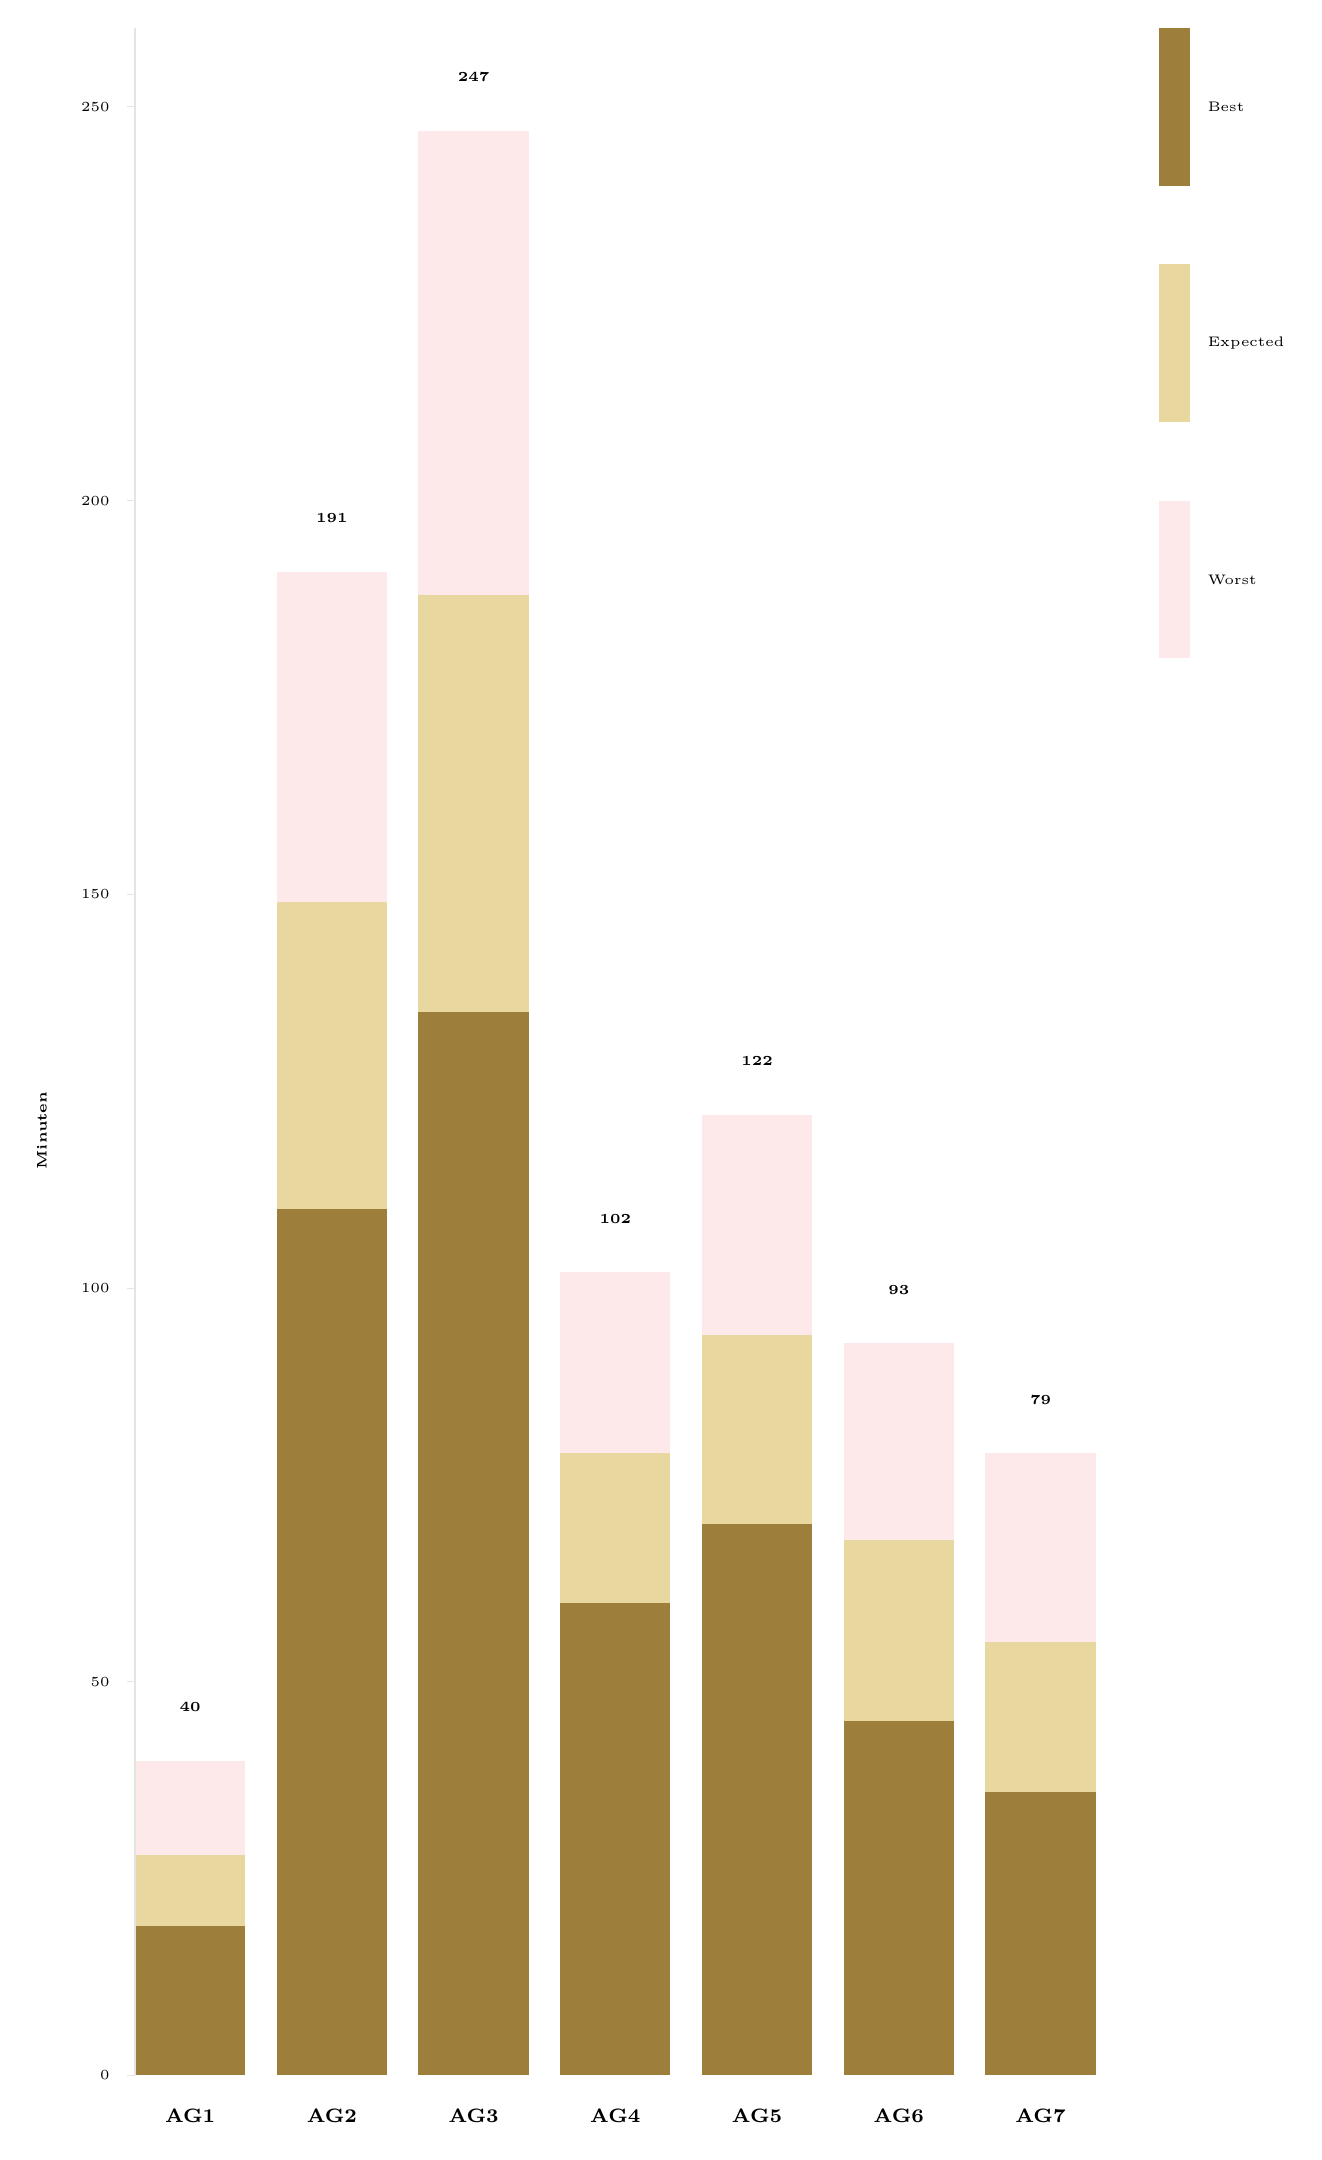
\begin{tikzpicture}
% Waterfall-style bar chart showing time distribution
\definecolor{bar1}{HTML}{b09a45}
\definecolor{bar2}{HTML}{c8aa50}
\definecolor{bar3}{HTML}{d4a853}
\foreach \i/\name/\best/\exp/\worst in {
  0/AG1/19/28/40,
  1/AG2/110/149/191,
  2/AG3/135/188/247,
  3/AG4/60/79/102,
  4/AG5/70/94/122,
  5/AG6/45/68/93,
  6/AG7/36/55/79
} {
  % Worst (background)
  \fill[riskredlight] (\i*18mm, 0) rectangle (\i*18mm+14mm, \worst/10);
  % Expected
  \fill[palegold] (\i*18mm, 0) rectangle (\i*18mm+14mm, \exp/10);
  % Best
  \fill[deepgold] (\i*18mm, 0) rectangle (\i*18mm+14mm, \best/10);
  % Label
  \node[font=\tiny\bfseries, anchor=south] at (\i*18mm+7mm, \worst/10+0.5) {\worst};
  \node[font=\scriptsize\bfseries, below] at (\i*18mm+7mm, -0.3) {\name};
}
% Y-axis
\draw[border] (0,0) -- (0,26);
\foreach \y/\lab in {0/0, 5/50, 10/100, 15/150, 20/200, 25/250} {
  \draw[border] (-1mm, \y) -- (0, \y);
  \node[font=\tiny, anchor=east] at (-2mm, \y) {\lab};
}
\node[font=\tiny\bfseries, rotate=90, anchor=south] at (-10mm, 12) {Minuten};
% Legend
\fill[deepgold] (130mm, 24) rectangle (134mm, 26); \node[font=\tiny, anchor=west] at (135mm, 25) {Best};
\fill[palegold] (130mm, 21) rectangle (134mm, 23); \node[font=\tiny, anchor=west] at (135mm, 22) {Expected};
\fill[riskredlight] (130mm, 18) rectangle (134mm, 20); \node[font=\tiny, anchor=west] at (135mm, 19) {Worst};
\end{tikzpicture}
\end{center}

{\footnotesize\color{textsecondary}\textbf{Lesehinweis:} Der dunkelste Bereich ist Best Case, der mittlere Expected, der helle Worst Case. AG3 (Oberseite) hat die größte Bandbreite → höchste Unsicherheit wegen geschätzter Taschengeometrien.}

\vspace{6pt}
\fcolorbox{gold}{palegold!20}{%
  \parbox{0.95\textwidth}{\footnotesize
    \textbf{Schnittdaten-Basis (S355, HB 180):} $v_c = 150$ m/min (Planfräsen), $v_c = 140$ m/min (Konturfräsen), $v_c = 80$ m/min (Bohren) · Quelle: Sandvik CoroPlus, Walter GPS · \textbf{Formel Hauptzeit:} $t_h = \frac{L \times n_{Bahnen}}{v_f} \times k_{Neben}$ mit $k_{Neben} = 1{,}15$ (Nebenzeiten 15\%)
  }%
}

\newpage

\sectiongold{8 \quad Optimaler Workflow: CNC Planner Pro + Arbeitsvorbereiter}

\vspace{4pt}
\begin{center}
\fcolorbox{gold}{palegold!20}{%
  \parbox{0.9\textwidth}{\centering\large\bfseries
    3 Phasen · 15 Minuten · ±10\% Genauigkeit
  }%
}
\end{center}
\vspace{8pt}

% --- Phase diagram ---
\begin{center}
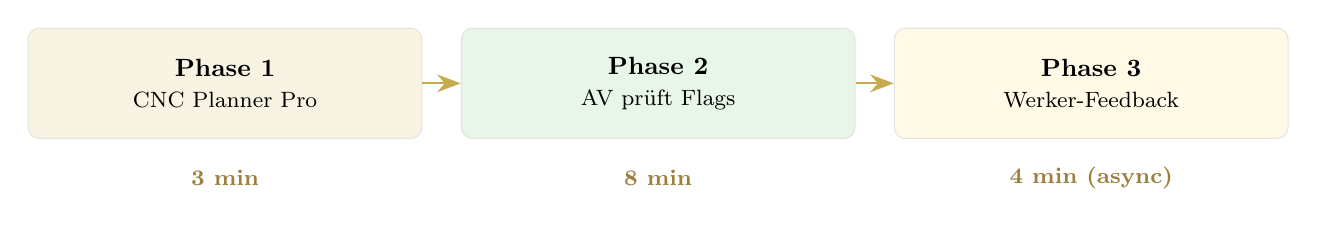
\begin{tikzpicture}[
  phase/.style={draw=border, fill=surface, rounded corners=4pt, minimum width=50mm, minimum height=14mm, align=center, font=\small},
  arrow/.style={-{Stealth[length=3mm]}, thick, color=gold},
  timelab/.style={font=\footnotesize\bfseries, color=deepgold},
]
\node[phase, fill=palegold!30] (p1) at (0,0) {\textbf{Phase 1}\\\footnotesize CNC Planner Pro};
\node[phase, fill=riskgreenlight] (p2) at (55mm,0) {\textbf{Phase 2}\\\footnotesize AV prüft Flags};
\node[phase, fill=riskyellowlight] (p3) at (110mm,0) {\textbf{Phase 3}\\\footnotesize Werker-Feedback};
\draw[arrow] (p1) -- (p2);
\draw[arrow] (p2) -- (p3);
\node[timelab] at (0,-12mm) {3 min};
\node[timelab] at (55mm,-12mm) {8 min};
\node[timelab] at (110mm,-12mm) {4 min (async)};
\end{tikzpicture}
\end{center}

\vspace{6pt}

\begin{tabularx}{\textwidth}{>{\bfseries\footnotesize}p{18mm} >{\footnotesize}X >{\footnotesize}r}
\toprule
\textbf{Phase} & \textbf{Was passiert} & \textbf{Dauer} \\
\midrule
\rowcolor{palegold!15}
Phase 1 & \textbf{CNC Planner:} PDF-Import → automatische Kalkulation mit REFA-Zeiten, Materialkosten, Zuschlägen. Ergebnis: Erstschätzung + Risiko-Flags. & 3 min \\
\rowcolor{riskgreenlight}
Phase 2 & \textbf{AV prüft nur die Flags:} Werkstoff korrekt? Aufspannungen realistisch? Rüstzeiten plausibel? Eigene BAB-Sätze eintragen. \textit{Rechnet nichts — validiert und korrigiert.} & 8 min \\
\rowcolor{riskyellowlight}
Phase 3 & \textbf{Werker-Validierung:} 📱 WhatsApp an Werker für 2–3 größte Zeitblöcke. Antwort fließt in Nachkalkulation → System lernt. & 4 min \\
\bottomrule
\end{tabularx}

\vspace{8pt}

\subsectiongold{Was der AV konkret prüft (Phase 2)}

\begin{tabularx}{\textwidth}{>{\footnotesize}p{5mm} >{\footnotesize}X >{\footnotesize}X >{\footnotesize}r}
\toprule
& \textbf{CNC Planner zeigt} & \textbf{AV macht} & \textbf{Zeit} \\
\midrule
1 & ⚠ Werkstoff unklar (S355/GJS) & Zeichnung → korrekten Werkstoff wählen & 30s \\
2 & ⚠ Materialpreis EUR 7,50/kg & Tagespreis bestätigen oder korrigieren & 30s \\
3 & ⚠ 4 Aufspannungen & ``3 reichen'' oder ``5 nötig wegen X'' & 1 min \\
4 & ⚠ Rüstzeit 35min Aufsp.\,1 & Bestätigen oder Erfahrungswert eintragen & 30s \\
5 & ⚠ Planfräsen 55min & ``Eher 45min mit unserem Ø100er'' & 30s \\
6 & 🔴 Brennschnitt inklusive? & Ja/Nein → Klick & 10s \\
7 & Zuschlagssätze (MGK, VwGK) & Eigene BAB-Sätze eintragen (einmalig) & 2 min \\
\bottomrule
\end{tabularx}

\vspace{8pt}

\subsectiongold{Vergleich: Heute vs. Optimiert}

\renewcommand{\arraystretch}{1.3}
\begin{tabularx}{\textwidth}{>{\bfseries}l X r r}
\toprule
\textbf{Methode} & \textbf{Beschreibung} & \textbf{Dauer} & \textbf{Genauigkeit} \\
\midrule
\rowcolor{riskredlight}
Heute & AV macht 100\% alleine (Zeichnung, Zeiten, BAB, Angebot) & 2–4h & ±15\% \\
\rowcolor{riskyellowlight}
Besser & CNC PP macht 80\%, AV prüft 20\% & 15 min & ±10\% \\
\rowcolor{riskgreenlight}
\textbf{Optimal} & \textbf{CNC PP + AV-Prüfung + Werker-Feedback} & \textbf{15 min} & \textbf{±8\%} \\
\bottomrule
\end{tabularx}
\renewcommand{\arraystretch}{1.0}

\vspace{4pt}
{\footnotesize\color{textsecondary} Der AV schafft damit \textbf{12 Kalkulationen pro Tag} statt 2–3. Bei einem durchschnittlichen Auftragswert von EUR 5.000 entspricht das einem Angebots-Durchsatz von EUR 60.000/Tag statt EUR 15.000/Tag.}

\vspace{10pt}

\fcolorbox{gold}{palegold!20}{%
  \parbox{0.95\textwidth}{%
    \textbf{Kernaussage:} Der CNC Planner ersetzt nicht den Arbeitsvorbereiter — er gibt ihm 80\% seiner Zeit zurück. Statt 3 Stunden zu rechnen, prüft er 8 Minuten.
  }%
}

% ============================================================
% SUMMARY & AUSBLICK
% ============================================================
\vspace{14pt}
\sectiongold{9 \quad Zusammenfassung}

\begin{itemize}[leftmargin=*, itemsep=3pt]
  \item \textbf{Basiskalkulation:} EUR 19.730/Stück (4 Stück = EUR 78.920 netto)
  \item \textbf{Reale Bandbreite:} EUR 14.200 – 26.800 je nach Werkstoff und Rohteil-Zustand
  \item \textbf{Größtes Risiko:} Werkstoff-Klärung S355 vs. GJS-700 (±EUR 8.000/Stk)
  \item \textbf{Fertigungszeit:} 661 min/Stück (11,0h) · 4 Aufspannungen · 11 Arbeitsgänge
  \item \textbf{Empfohlene Angebotsstrategie:} Getrennte Positionen (Material + Bearbeitung + Einrichtung)
  \item \textbf{Kalkulations\-dauer:} 1–3 min (CNC Planner Pro) statt 2–4h (manuell) = \textbf{95\% Zeitersparnis}
\end{itemize}

\newpage

% ============================================================
% ZUKUNFT
% ============================================================
\sectiongold{10 \quad Warum CNC Planner Pro der beste Weg ist}

\subsectiongold{Das Problem heute}

\begin{center}
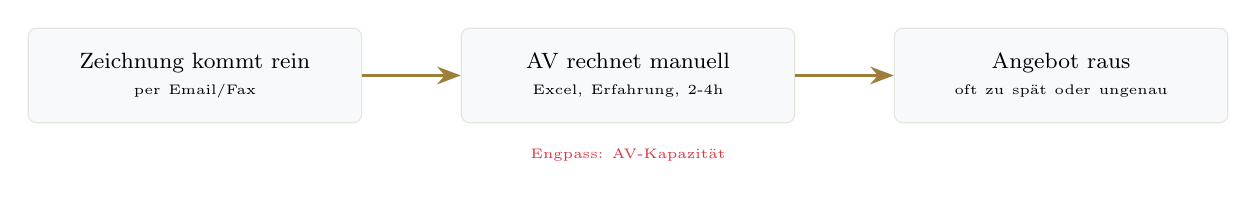
\begin{tikzpicture}[
  block/.style={rectangle, draw=border, fill=riskgray, rounded corners=3pt, minimum width=42mm, minimum height=12mm, font=\footnotesize, text width=40mm, align=center},
  arrow/.style={-{Stealth[length=3mm]}, thick, color=deepgold}
]
\node[block] (a) at (0,0) {Zeichnung kommt rein\\{\tiny per Email/Fax}};
\node[block] (b) at (55mm,0) {AV rechnet manuell\\{\tiny Excel, Erfahrung, 2-4h}};
\node[block] (c) at (110mm,0) {Angebot raus\\{\tiny oft zu spät oder ungenau}};
\draw[arrow] (a) -- (b);
\draw[arrow] (b) -- (c);
\node[font=\tiny\color{riskred}, below=2mm of b] {Engpass: AV-Kapazität};
\end{tikzpicture}
\end{center}

\vspace{4pt}
{\footnotesize
\textbf{Typische Probleme in der Arbeitsvorbereitung:}
\begin{itemize}[leftmargin=*, itemsep=2pt]
  \item Kalkulation dauert 2–4 Stunden pro Anfrage → bei 5 Anfragen/Tag = AV ist Vollzeit nur am Kalkulieren
  \item Erfahrungswissen im Kopf des Meisters → nicht übertragbar, geht bei Ruhestand verloren
  \item Keine systematische Nachkalkulation → gleiche Fehler wiederholen sich
  \item Materialpreise veraltet → Angebote zu niedrig → Deckungsbeitrag schrumpft
\end{itemize}
}

\subsectiongold{Die Lösung: CNC Planner Pro als digitaler Arbeitsvorbereiter}

\begin{center}

\begin{tikzpicture}[
  block/.style={rectangle, draw=border, fill=riskgray, rounded corners=3pt, minimum width=36mm, minimum height=12mm, font=\footnotesize, text width=34mm, align=center},
  goldblock/.style={rectangle, draw=gold, fill=palegold!30, rounded corners=3pt, minimum width=36mm, minimum height=12mm, font=\footnotesize\bfseries, text width=34mm, align=center},
  arrow/.style={-{Stealth[length=3mm]}, thick, color=deepgold}
]
\node[block] (a) at (0,0) {Zeichnung\\{\tiny PDF/STEP}};
\node[goldblock] (b) at (42mm,0) {CNC Planner Pro\\{\tiny 1-3 min, REFA-basiert}};
\node[block] (c) at (84mm,0) {AV prüft\\{\tiny 10-15 min}};
\node[block] (d) at (126mm,0) {Angebot\\{\tiny fundiert, schnell}};
\draw[arrow] (a) -- (b);
\draw[arrow] (b) -- (c);
\draw[arrow] (c) -- (d);
\node[font=\tiny\color{riskgreen}, below=2mm of b] {95\% schneller};
\end{tikzpicture}
\end{center}

\subsectiongold{Roadmap — Was kommt als Nächstes}

\begin{tabularx}{\textwidth}{>{\bfseries\footnotesize}p{6mm} >{\footnotesize}p{28mm} >{\footnotesize}X >{\footnotesize}p{30mm}}
\toprule
& \textbf{Feature} & \textbf{Was bringt das?} & \textbf{Nutzen für den Betrieb} \\
\midrule
\rowcolor{riskgreenlight}
\circled{1} & \textbf{Prüfprotokoll} & System fragt aktiv nach fehlenden Infos (Werkstoff, Rohteil, Toleranzen) — wie ein erfahrener AV-Meister & Weniger Rückfragen, weniger Fehler \\
\circled{2} & \textbf{STEP-Import} & 3D-Modell einlesen → exakte Volumen, Features automatisch erkennen & Material ±5\% statt ±20\% \\
\rowcolor{riskgreenlight}
\circled{3} & \textbf{Eigene Stundensätze} & BAB einmalig hinterlegen → betriebsspezifische Kalkulation & Kein Anpassen mehr nötig \\
\circled{4} & \textbf{Nachkalkulation} & Ist vs. Soll: Was hat wirklich gedauert? → System lernt & Jedes Teil macht den nächsten Preis besser \\
\rowcolor{riskgreenlight}
\circled{5} & \textbf{Werker-Feedback} & Meister korrigiert Zeiten per Handy → fließt in Datenbank & Erfahrungswissen wird digital gesichert \\
\circled{6} & \textbf{Maschinenpark} & Welche Maschine passt am besten? → Verfahrwege, Spindel, Auslastung & Optimale Auslastung, weniger Stillstand \\
\rowcolor{riskgreenlight}
\circled{7} & \textbf{Feature Recognition} & KI erkennt Taschen, Bohrungen, Konturen aus STEP → Zeiten pro Feature & Vollautomatische Vorkalkulation \\
\bottomrule
\end{tabularx}

\vspace{10pt}

\subsectiongold{Der entscheidende Vorteil}

\begin{center}
\fcolorbox{gold}{palegold!20}{%
  \parbox{0.9\textwidth}{\centering
    \large\bfseries Das System wird mit jeder Kalkulation besser.\\[6pt]
    \normalsize\normalfont\color{textsecondary} 
    Heute: ±20\% Genauigkeit (Richtwerte) → Mit AV-Prüfung: ±10\%\\
    Mit Nachkalkulation: ±5\% → Mit Feature Recognition: Vollautomatisch\\[6pt]
    \textbf{Das Wissen des Meisters geht nicht in Rente — es bleibt im System.}
  }%
}
\end{center}

\vspace{8pt}

{\footnotesize\color{textsecondary}
\textbf{Warum jetzt?} Die KI-Technologie ist reif genug, um REFA-basierte Kalkulationen in Minuten zu erstellen — aber noch jung genug, dass Vorreiter einen echten Wettbewerbsvorteil aufbauen. Wer als erster seine Erfahrungswerte digitalisiert, hat einen Vorsprung, den Nachzügler nicht aufholen können.
}

% ============================================================
% FOOTER
% ============================================================
\vfill

\begin{center}
{\color{gold}\rule{0.6\textwidth}{1pt}}\\[8pt]
{\footnotesize\color{textsecondary}
Erstellt: 2026-02-10 · CNC Planner Pro (AI-Assisted)\\
Gültigkeit: Bis Klärung der offenen Fragen · Materialpreise tagesaktuell prüfen\\
Klassifizierung: ⚠ INTERN — Basis für Angebotserstellung\\[4pt]
\textbf{Ainary Consulting} · florian@ainaryventures.com
}
\end{center}

\end{document}
